\begin{frame}{Datos y preprocesamiento adaptado al dataset UCI}
    \begin{itemize}
        \item \textbf{Fuente:} ElectricityLoadDiagrams20112014 (UCI), adoptado tras inconsistencias estructurales en los metadatos de UNICON.
        \item \textbf{Matriz de análisis (X):} Agregación de carga total simulando un campus. Las filas representan días y las columnas corresponden a 96 franjas de consumo (cada 15 minutos).
        \item \textbf{Contexto:} Debido a la ausencia de variables meteorológicas en UCI, la variable contextual utilizada es exclusivamente un indicador binario de fin de semana.
        \item \textbf{Preprocesamiento:} Descarte de días incompletos y estandarización Z-score (media 0, desviación 1) por columna para asegurar equidad en la varianza geométrica.
    \end{itemize}
\end{frame}

\begin{frame}{Resultados cuantitativos: Varianza explicada por PCA}
    \begin{columns}
        \begin{column}{0.5\textwidth}
            \begin{itemize}
                \item El modelo se ajustó para retener al menos el 90\% de la varianza.
                \item Un solo componente principal ($k=1$) fue suficiente para capturar la estructura dominante.
                \item El PC1 explica el \textbf{92.71\%} de la varianza total de los datos.
            \end{itemize}
        \end{column}
        \begin{column}{0.5\textwidth}
            \begin{figure}
                \centering
                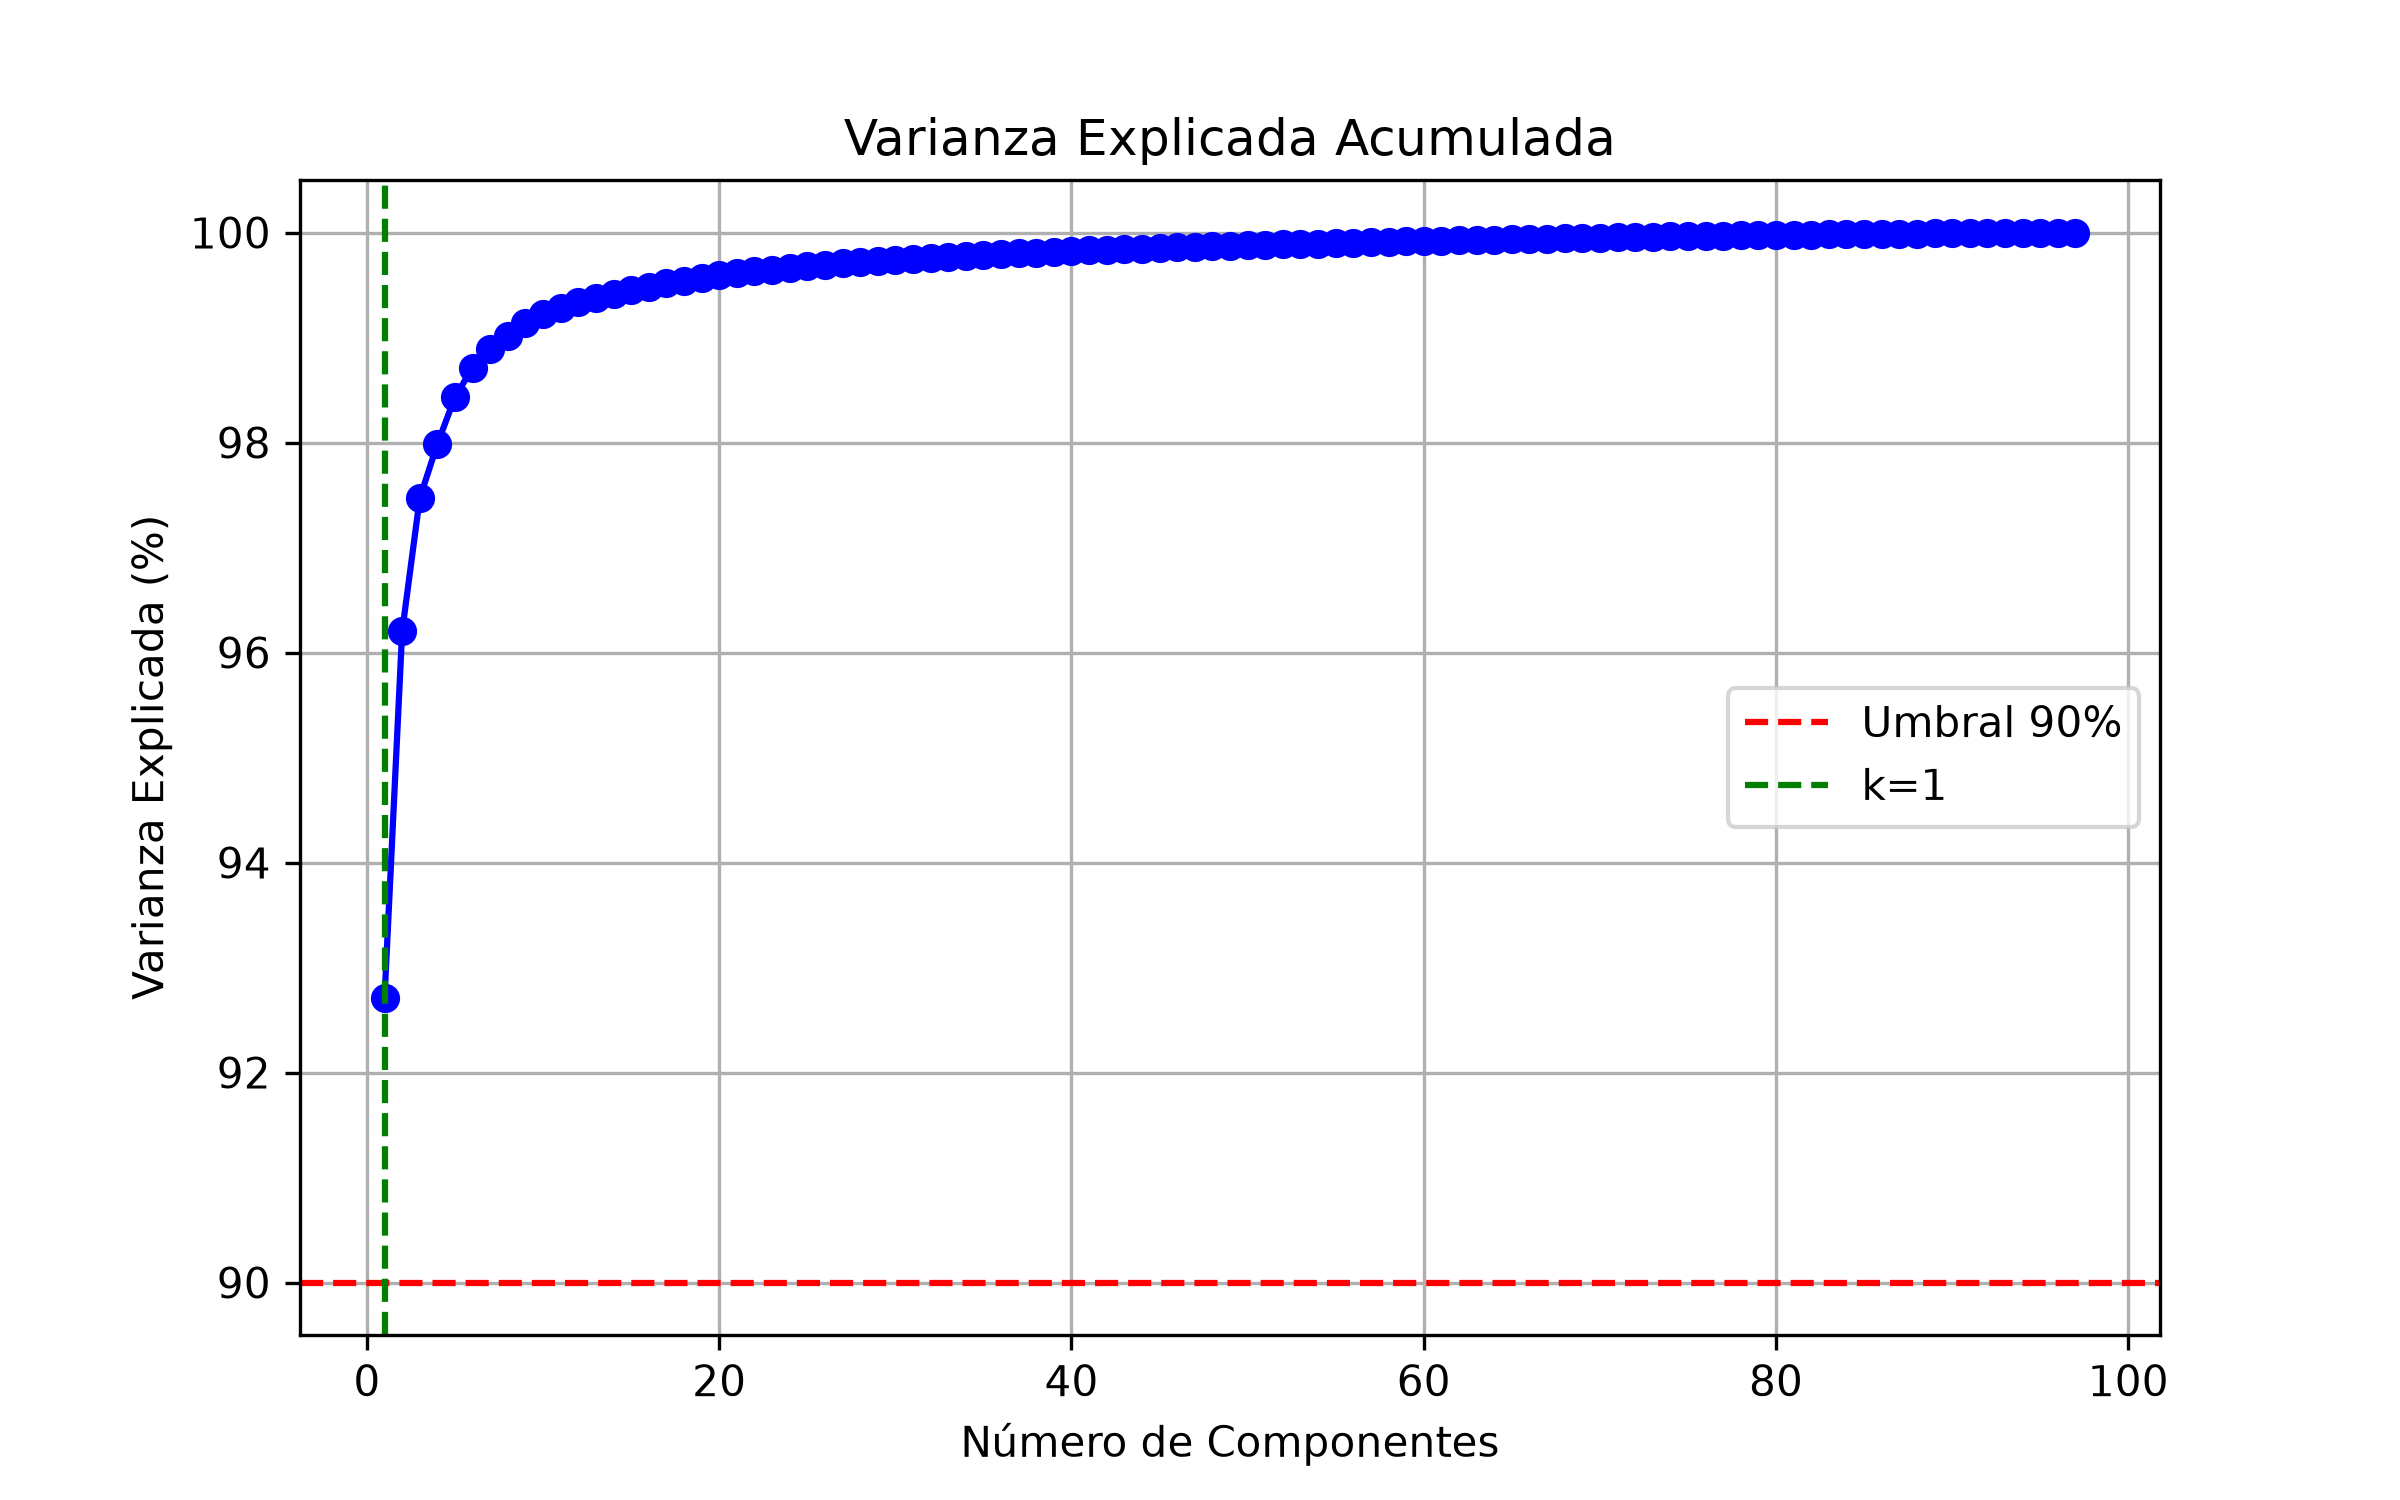
\includegraphics[width=\textwidth]{figuras/varianza_explicada.png}
                \caption{Varianza explicada acumulada}
            \end{figure}
        \end{column}
    \end{columns}
\end{frame}

\begin{frame}{Resultados cuantitativos: Detección vs Línea base}
    \begin{columns}
        \begin{column}{0.5\textwidth}
            \begin{itemize}
                \item \textbf{PCA (Percentil 99):} Detectó 30 días únicos anómalos.
                \item 15 días superaron el umbral del estadístico $T^2$ (distancia en el hiperplano).
                \item 15 días superaron el umbral de SPE (error de reconstrucción).
                \item \textbf{Línea base ($|z| > 3$):} Detectó 1 día anómalo.
                \item \textbf{Coincidencia:} Hubo 1 día detectado por ambos métodos.
            \end{itemize}
        \end{column}
        \begin{column}{0.5\textwidth}
            \begin{figure}
                \centering
                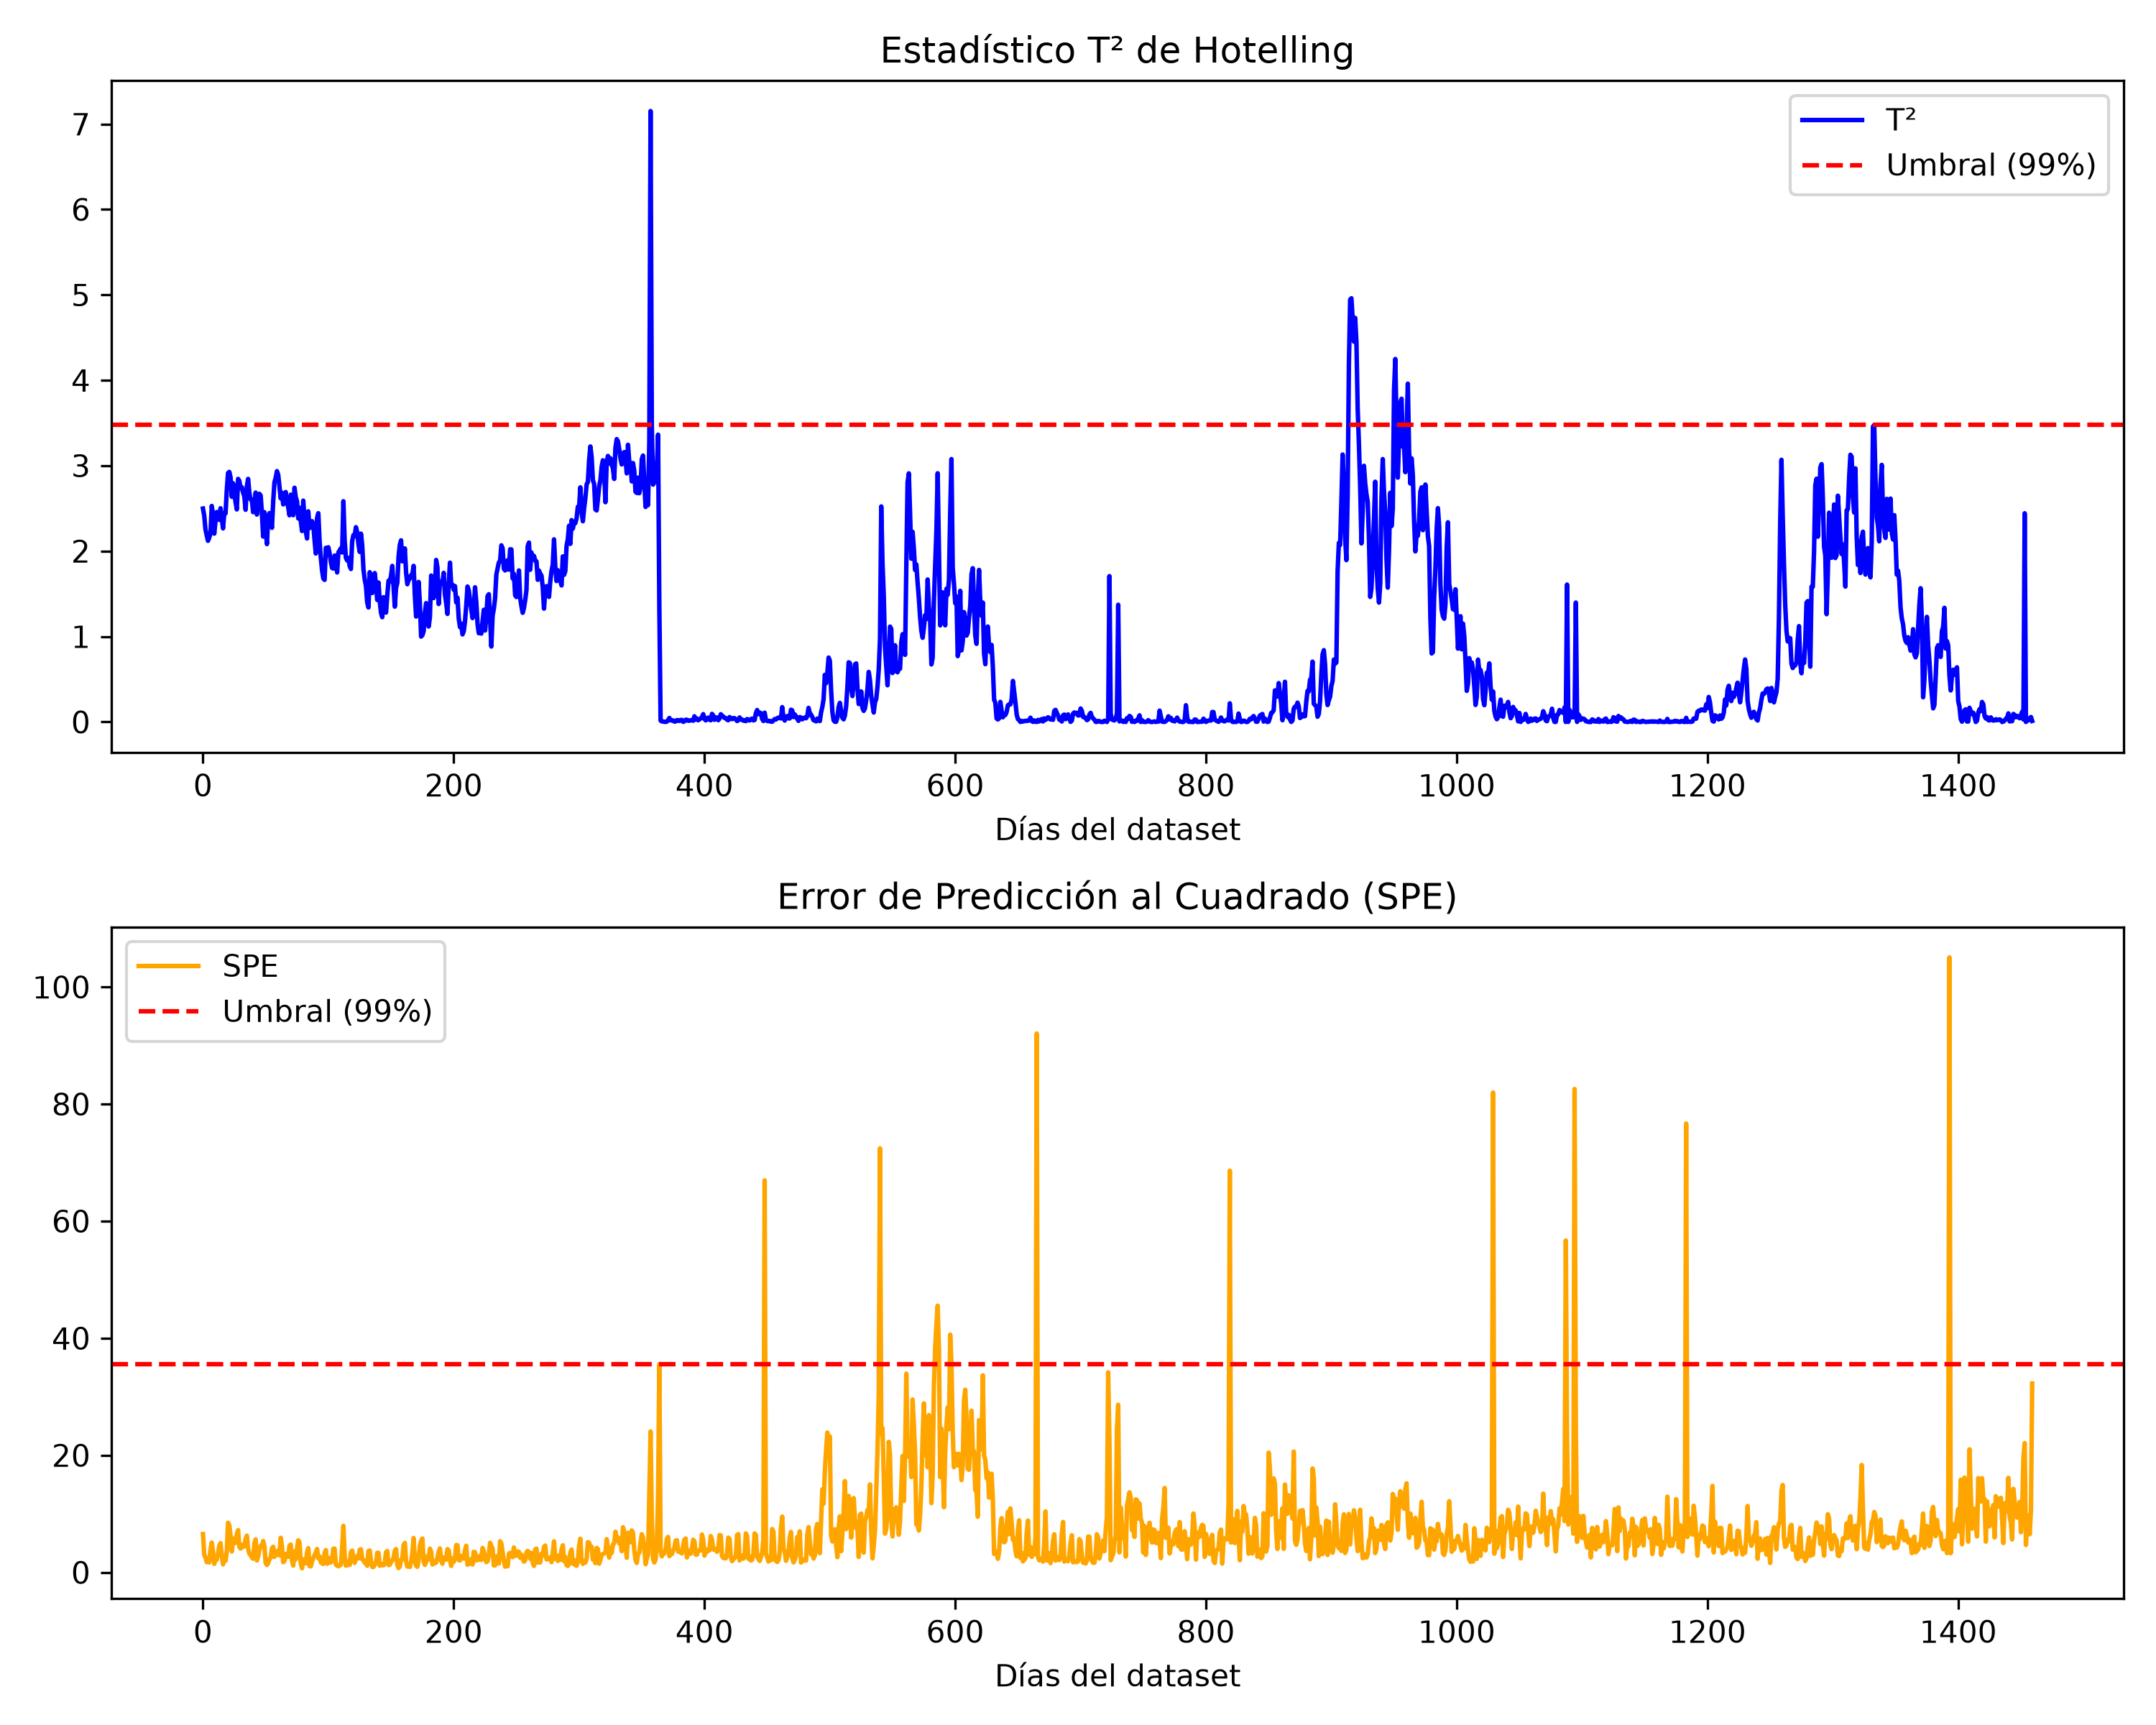
\includegraphics[width=\textwidth]{figuras/estadisticos_t2_spe.png}
                \caption{Estadísticos $T^2$ y SPE}
            \end{figure}
        \end{column}
    \end{columns}
\end{frame}

\begin{frame}{Resultados cualitativos: Proyección 2D del consumo}
    \begin{columns}
        \begin{column}{0.5\textwidth}
            \begin{itemize}
                \item La proyección de los datos sobre los dos primeros componentes principales muestra una clara estructura de agrupación.
                \item Las observaciones anómalas (marcadas en rojo) se separan efectivamente de la nube de datos dominante de los días normales.
                \item Las desviaciones extremas en el eje PC1 reflejan anomalías de magnitud global, mientras que las de PC2 indican alteraciones en el patrón de la curva diaria.
            \end{itemize}
        \end{column}
        \begin{column}{0.5\textwidth}
            \begin{figure}
                \centering
                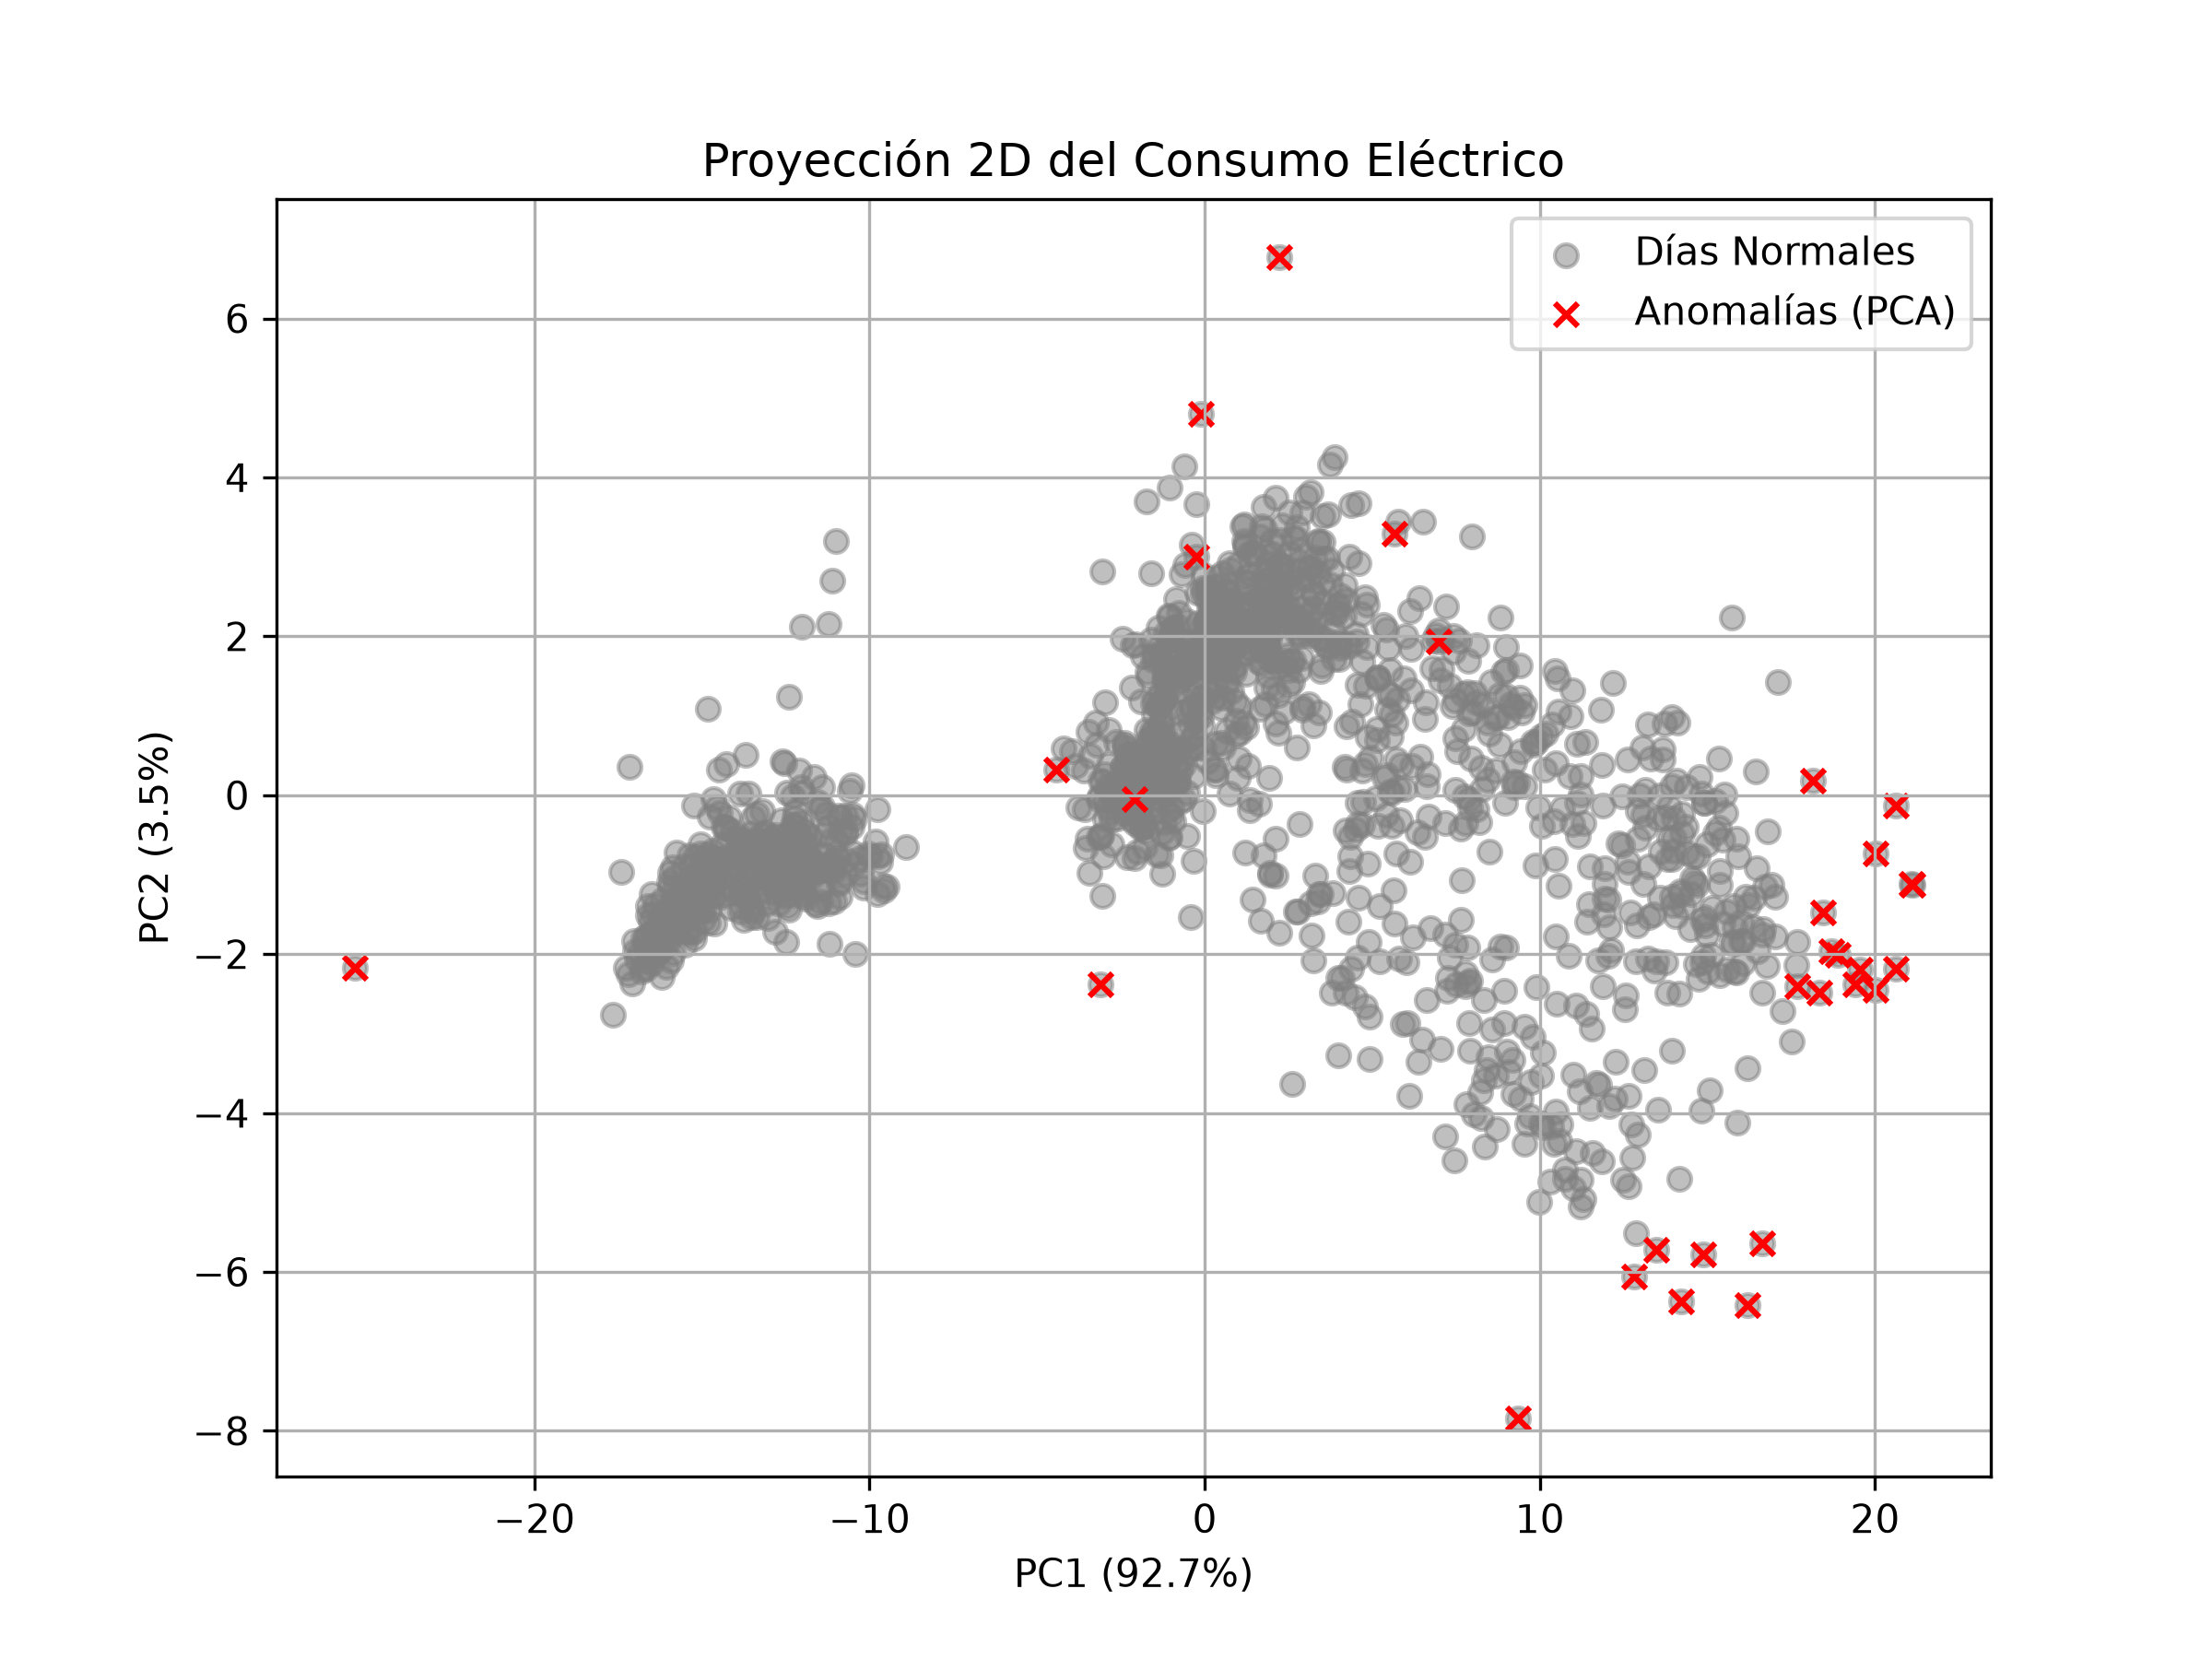
\includegraphics[width=\textwidth]{figuras/proyeccion_2d.png}
                \caption{Proyección sobre PC1 y PC2}
            \end{figure}
        \end{column}
    \end{columns}
\end{frame}

\begin{frame}{Discusión y limitaciones de la prueba de concepto}
    \begin{itemize}
        \item \textbf{Limitación principal:} El dataset no contiene etiquetas reales (*ground truth*) de fallas eléctricas o eventos inusuales validados por la administración.
        \item Por lo anterior, \textbf{no se calculan métricas de clasificación tradicionales} como \textit{Precisión} o \textit{Recall}.
        \item La validación se apoya en el consenso técnico (comparación empírica contra la línea base estadística) y la separación visual en el espacio latente.
        \item El cambio de emergencia al dataset de UCI restringió la evaluación del contexto climático (temperatura y humedad), limitando la interpretación semántica de las anomalías detectadas.
    \end{itemize}
\end{frame}

\begin{frame}{Conclusiones y trabajo futuro}
    \begin{itemize}
        \item PCA demuestra ser un enfoque no supervisado eficiente para abstraer el 92.71\% del comportamiento energético de un campus en una sola dimensión ($k=1$).
        \item Los estadísticos $T^2$ y SPE separan con éxito variaciones extremas en magnitud y forma de onda respecto al comportamiento habitual del dataset.
        \item \textbf{Trabajo futuro:} Integrar datasets con variables meteorológicas puras (temperatura, radiación, humedad) para discriminar si un consumo atípico es una anomalía genuina o una simple respuesta térmica del edificio.
    \end{itemize}
\end{frame}